\documentclass[11pt]{article}
\usepackage[margin=1in]{geometry}
\usepackage{amsmath}
\usepackage{graphicx}
\usepackage{booktabs}
\usepackage{siunitx}
\usepackage[hidelinks]{hyperref}
\usepackage{caption}
\graphicspath{{../figures/}{figures/}}
\sisetup{group-separator={,}, group-minimum-digits=4}
\captionsetup{font=small, labelfont=bf}

\title{Does Wan2.1's Cost Grow the Way the FLOP Count Says?\\
\large Forward-pass latency and memory versus video token count on a Tesla T4}
\author{Thomas Liu}
\date{November 2026}

\begin{document}
\maketitle

\section{Question}

Text-to-video models are slow, and the usual explanation is that self-attention is quadratic in sequence length. I wanted to check how much of the real cost that explanation accounts for. My question was: \emph{how closely do prefill latency and memory scale with prompt length, compared with what a FLOP count and a memory count predict?}

I used Wan2.1-T2V-1.3B \cite{wan}, the small open text-to-video model from Alibaba, on a free Google Colab Tesla T4 (\SI{15.6}{GB}, half precision). Two terms need redefining for a video diffusion model. The text prompt is always padded to 512 tokens, so the sequence that changes is the video itself: ``prompt length'' here is $N$, the number of video latent tokens. ``Prefill'' is one forward pass of the diffusion transformer, which is one denoising step. A full video needs about 50 of them.

Before running anything I wrote down two hypotheses.
\begin{enumerate}
\item Latency follows the shape of the FLOP model, close to linear in $N$ at first and bending toward quadratic near $N \approx \num{14000}$, but sits well above the hardware's compute limit, and efficiency drops once attention dominates.
\item With a fused attention kernel, activation memory is linear in $N$ and within about $1.5\times$ of my formula. With naive attention it is quadratic and above the formula.
\end{enumerate}

\section{The architecture, and why it is built this way}

Wan2.1 has three parts \cite{wan}. A umT5 text encoder runs once per prompt and outputs a $512 \times 4096$ embedding. A 3D causal VAE compresses the video by $4\times$ in time and $8\times 8$ in space into 16 latent channels, so 81 frames at $480 \times 832$ become a $21 \times 60 \times 104$ latent. A diffusion transformer (DiT), trained with flow matching, denoises that latent. Only the DiT runs at every step, so it is the part I benchmarked. The loaded checkpoint reports 30 layers, hidden size $d = 1536$, 12 heads of dimension 128, feed-forward size $f = 8960$, a $1\times2\times2$ patch embedding, and \num{1.42}~billion parameters.

Three design choices decide how cost scales.
\begin{itemize}
\item \textbf{Compress first.} The VAE and the patch embedding together turn each $4 \times 16 \times 16$ block of pixels into one token. The authors work in this latent space because attention over raw pixels would be far too expensive. It also fixes the token count: $N = F_\ell \cdot (H_\ell/2)(W_\ell/2)$, or \num{1560} tokens per latent frame at 480p and \num{32760} for a standard 81-frame clip.
\item \textbf{Full spatio-temporal self-attention.} Every token attends to every other token across space and time, instead of using separate spatial and temporal attention. This is what lets the model keep motion coherent over the whole clip, and it is the source of the $N^2$ term.
\item \textbf{Text enters through cross-attention.} Each block attends from the $N$ video tokens to the 512 text tokens. That cost is linear in $N$, so the text prompt adds a fixed per-token charge and never contributes a quadratic term.
\end{itemize}

\section{Predictions}

Counting two FLOPs per multiply-add, one block costs $8Nd^2$ for the self-attention projections, $4N^2d$ for the attention scores and weighted sum, $4Nd^2 + 4NLd$ for cross-attention on the video side, $4Ld^2$ for projecting the $L = 512$ text tokens, and $4Ndf$ for the feed-forward network. Over 30 blocks:
\begin{equation}
F(N) \approx 2.60\times10^{9}\,N + 1.84\times10^{5}\,N^{2} + 1.45\times10^{11}\ \text{FLOPs}.
\end{equation}
The quadratic term overtakes the rest at $N \approx \num{14100}$. For an 81-frame clip, $F = \SI{283}{TFLOP}$ per step and attention is 70\% of it. I ignored normalisation layers, the patch embedding and the timestep MLP.

For memory I assumed inference only (no stored activations for backprop), 2 bytes per value, and a peak set by the feed-forward hidden layer plus about six $d$-wide temporaries per token:
\begin{equation}
M_\text{fused}(N) \approx 2N(f + 6d) = \SI{36.4}{kB}\times N, \qquad
M_\text{naive}(N) \approx M_\text{fused}(N) + 48N^{2}\ \text{bytes}.
\end{equation}
The naive term is one $N \times N$ score matrix per head, counted twice for the scores and the softmax output. The $6d$ is a guess, so I expected the slope to be right and the constant to be off.

Between runs I expected latency to move with whatever else the shared Colab GPU was doing, mostly at small $N$ where a pass takes under \SI{0.1}{s}. I expected memory not to move at all.

\section{Method}

\textbf{Independent variable.} $N$, set by sweeping latent frames over $\{1,2,3,4,6,8,11,14,17,21,28,36\}$ at $60 \times 104$, plus two smaller single-frame shapes, giving 14 sizes from 104 to \num{56160} tokens.

\textbf{Dependent variables.} Latency of one DiT forward pass, timed with \texttt{torch.cuda.Event} and a synchronise, and peak activation memory, taken as \texttt{max\_memory\_allocated} minus the memory held by the weights (\SI{2.85}{GB}).

\textbf{Held constant.} Batch size 1, 512 text tokens, timestep 500, random latents and text embeddings, \texttt{torch.inference\_mode}, fp16 (the T4 does not support bf16), PyTorch 2.14.1+cu130, one Tesla T4.

\textbf{Model revision.} \texttt{Wan-AI/Wan2.1-T2V-1.3B-Diffusers}, \texttt{transformer} subfolder, \texttt{main} branch. I did not pin or log the commit hash; the repository README shows how to record it on a rerun.

\textbf{Timed runs.} Each size got 2 warm-up passes and 5 timed passes, and I report the median. The fused-attention sweep was run twice in the same session: run A covers the 11 sizes up to $N = \num{26520}$ and run B covers all 14. The three largest sizes, the naive-attention sweep and the same-$N$ check therefore have one run each.

\textbf{Conditions.} (i) PyTorch's default scaled-dot-product attention, which picks a fused kernel; (ii) the \texttt{MATH} backend, which builds the full $N \times N$ matrix; (iii) three different shapes that all give $N = \num{6240}$.

\section{Results}

Table~\ref{tab:raw} holds the raw numbers and Figures~\ref{fig:lat}--\ref{fig:var} plot them. The same data is in \texttt{data/results.csv} in the repository.

\begin{table}[htbp]
\centering
\footnotesize\setlength{\tabcolsep}{4pt}
\begin{tabular}{S[table-format=5.0] S[table-format=2.4] S[table-format=3.4] S[table-format=2.1] S[table-format=2.1] S[table-format=1.4] S[table-format=1.2] S[table-format=2.4] S[table-format=1.2]}
\toprule
& \multicolumn{5}{c}{Fused attention} & & \multicolumn{2}{c}{Naive attention} \\
\cmidrule(lr){2-6}\cmidrule(lr){8-9}
{$N$} & {Run A (s)} & {Run B (s)} & {Diff.\ (\%)} & {MFU (\%)} & {Mem.\ (GB)} & {Mem./model} & {Latency (s)} & {Mem.\ (GB)} \\
\midrule
104   & 0.0519  & 0.0810   & 43.8 & 9.7  & 0.0133 & 3.52 & 0.0701  & 0.02 \\
390   & 0.0857  & 0.0973   & 12.7 & 19.9 & 0.0279 & 1.97 & 0.1383  & 0.05 \\
1560  & 0.2986  & 0.3405   & 13.1 & 22.3 & 0.0830 & 1.46 & 0.6186  & 0.33 \\
3120  & 0.6600  & 0.7839   & 17.2 & 21.4 & 0.1617 & 1.43 & 1.8258  & 1.19 \\
4680  & 1.0708  & 1.2144   & 12.6 & 22.0 & 0.2382 & 1.40 & 3.3727  & 2.57 \\
6240  & 1.6667  & 1.8215   & 8.9  & 20.7 & 0.3136 & 1.38 & 5.6142  & 4.47 \\
9360  & 2.9008  & 3.1011   & 6.7  & 20.8 & 0.4699 & 1.38 & 12.8252 & 9.86 \\
12480 & 4.5816  & 4.8603   & 5.9  & 20.0 & 0.6238 & 1.37 & {OOM}   & {OOM} \\
17160 & 7.9180  & 8.1325   & 2.7  & 19.0 & 0.8537 & 1.37 & {--}    & {--} \\
21840 & 12.3562 & 12.4396  & 0.7  & 18.0 & 1.0840 & 1.37 & {--}    & {--} \\
26520 & 17.8531 & 17.8332  & 0.1  & 17.1 & 1.3159 & 1.36 & {--}    & {--} \\
32760 & {--}    & 28.5999  & {--} & 15.2 & 1.6209 & 1.36 & {--}    & {--} \\
43680 & {--}    & 57.0699  & {--} & 12.5 & 2.1602 & 1.36 & {--}    & {--} \\
56160 & {--}    & 100.1684 & {--} & 11.2 & 2.7763 & 1.36 & {--}    & {--} \\
\bottomrule
\end{tabular}
\caption{Raw results. Latencies are medians of 5 timed passes. Diff.\ is $|A-B|$ over the mean of A and B. MFU is achieved FLOP rate, from the mean latency, as a share of the T4's \SI{65}{TFLOP\per\second} peak. Memory was identical in both runs. Naive attention ran out of memory (OOM) at $N = \num{12480}$ and the sweep stopped there.}
\label{tab:raw}
\end{table}

\begin{figure}[htbp]
\centering
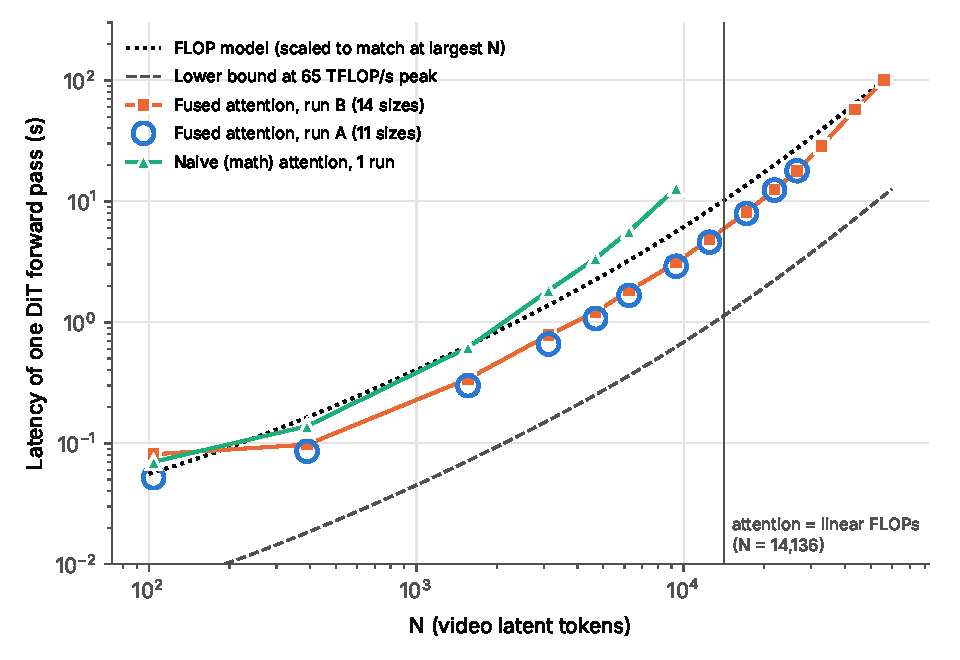
\includegraphics[width=0.78\linewidth]{fig1_latency_vs_tokens}
\caption{Latency of one forward pass against token count, both axes logarithmic. Open circles are run A, squares run B.}
\label{fig:lat}
\end{figure}

\begin{figure}[htbp]
\centering
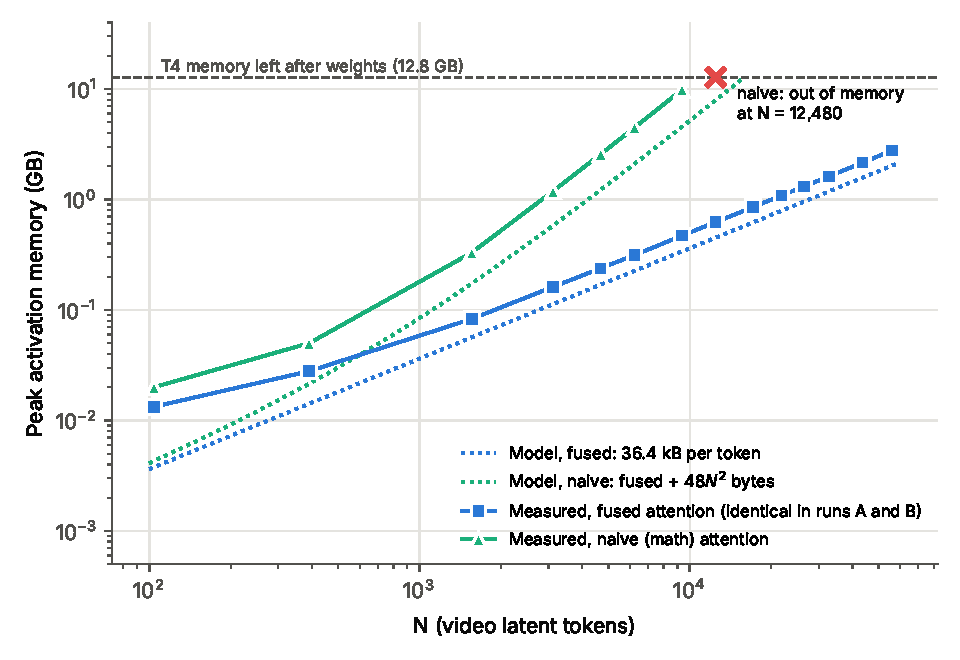
\includegraphics[width=0.78\linewidth]{fig2_memory_vs_tokens}
\caption{Peak activation memory against token count for both attention backends, with the two memory formulas.}
\label{fig:mem}
\end{figure}

\begin{figure}[htbp]
\centering
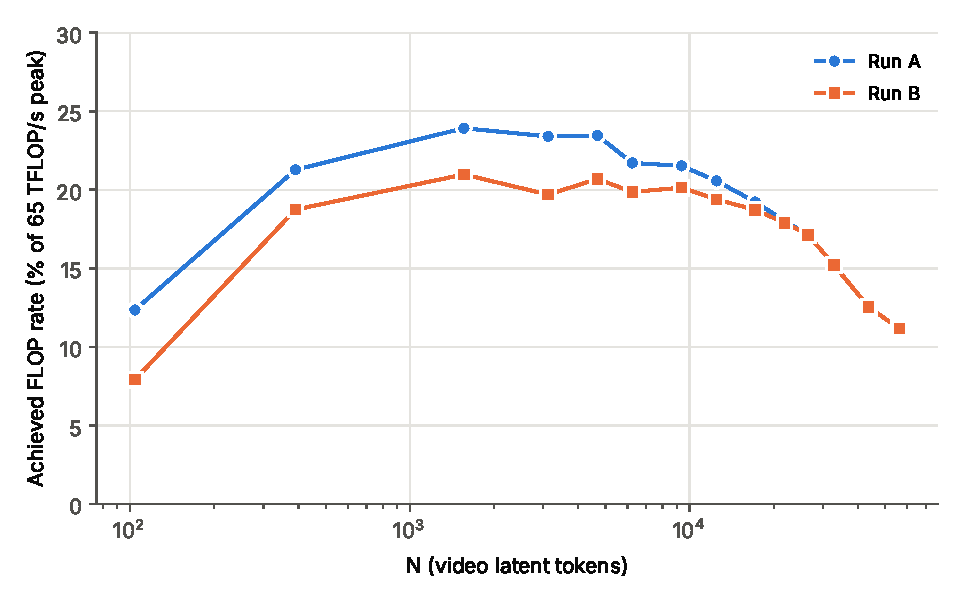
\includegraphics[width=0.78\linewidth]{fig3_utilisation_vs_tokens}
\caption{Achieved FLOP rate as a percentage of the T4's peak, for each run separately.}
\label{fig:mfu}
\end{figure}

\begin{figure}[htbp]
\centering
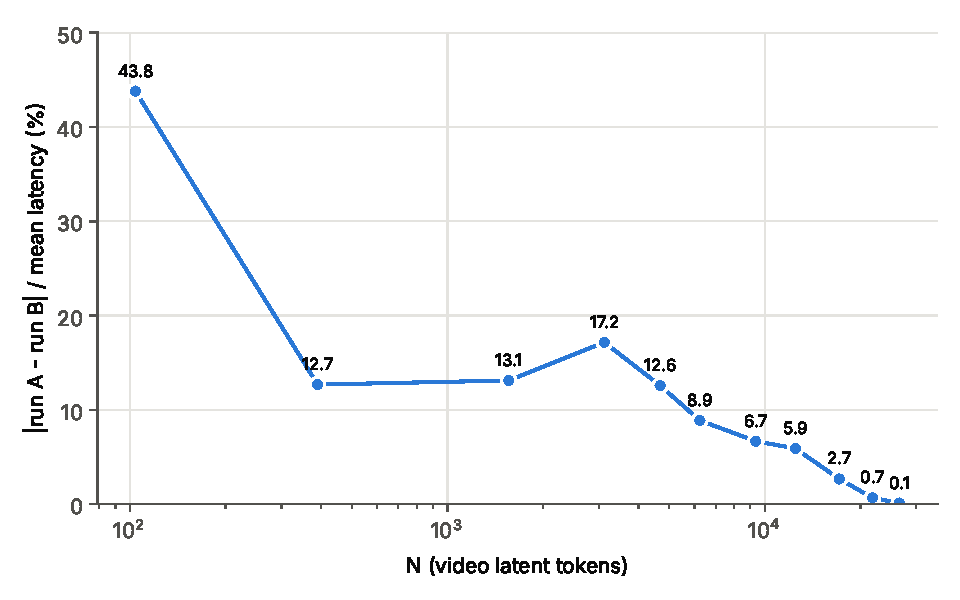
\includegraphics[width=0.78\linewidth]{fig4_run_to_run_variation}
\caption{Difference between run A and run B at each size measured twice, as a percentage of their mean.}
\label{fig:var}
\end{figure}

\textbf{Latency.} From $N = \num{1560}$ to \num{12480} the measured log-log slope is 1.29 against 1.24 from the FLOP model, and the GPU holds a steady 20--22\% of peak. Past the crossover the curve bends upward as predicted, but too far: from \num{12480} to \num{56160} the measured slope is 2.05 against a predicted 1.65, and across the top three sizes it is 2.33, which is steeper than quadratic. Utilisation falls from 20\% to 11\% over the same range (Figure~\ref{fig:mfu}). If the T4 had kept the \SI{14}{TFLOP\per\second} it achieved in the middle of the sweep, the largest size would have taken about \SI{52}{s}. It took \SI{100}{s}. One step of a standard 81-frame clip took \SI{28.6}{s}.

\textbf{Memory.} With fused attention, memory is linear (slope 0.98 for $N \ge \num{1560}$) at \SI{49.4}{kB} per token, a constant $1.36$--$1.46\times$ my formula. Below \num{1560} tokens the ratio is 2--3.5 because a few megabytes of fixed overhead dominate. With naive attention the slope is 1.89 and memory is about $2.1\times$ the formula. That factor matters: the formula predicted \SI{7.9}{GB} at $N = \num{12480}$, which would have fit in the \SI{12.8}{GB} left after the weights, but the run failed there. Naive attention was also 1.8 to 4.1 times slower than fused.

\textbf{Same $N$, different shape.} The shapes $4\times60\times104$, $8\times30\times104$ and $16\times30\times52$ took \SI{1.823}{s}, \SI{1.822}{s} and \SI{1.826}{s}, a 0.2\% spread, with identical memory. Only the token count matters, not how it splits between frames and resolution.

\textbf{Variation across runs.} The two runs differ by 44\% at $N = 104$, 9--17\% from 390 to \num{6240} tokens, and under 3\% from \num{17160} up, reaching 0.1\% at \num{26520} (Figure~\ref{fig:var}). Run A was the faster one in 10 of the 11 pairs, so this looks like a shift in the GPU's state between passes more than random noise. Memory matched to every reported digit.

\section{Back to the question}

Hypothesis 1 held in part. The FLOP count predicts the shape of the latency curve up to about \num{12000} tokens and predicts where it bends. It does not predict how hard it bends. At large $N$ the measured cost grows faster than the FLOPs, so a FLOP model fitted on short clips underestimates a long clip by nearly a factor of two. The run also stayed 4.5 to 10 times above the compute lower bound throughout, as expected.

Hypothesis 2 held. Fused-attention memory is linear and within $1.5\times$ of the formula above \num{1560} tokens, and naive attention is close to quadratic and about twice the formula. On this GPU memory never limited the fused path: \num{56160} tokens needed \SI{2.8}{GB}. Time is the constraint.

Several things limit these conclusions.
\begin{itemize}
\item \textbf{Two runs, not three, and one at the top.} The sizes where the model fails worst, \num{32760} to \num{56160} tokens, were measured once. The agreement at \num{26520} (0.1\%) suggests long passes are stable, but that is an inference.
\item \textbf{No within-run spread.} The notebook computes a standard deviation over the 5 timed passes, but the only one that survives in the saved output is the smoke test (\SI{1.5}{ms} on \SI{85}{ms}).
\item \textbf{One GPU, one precision, unpinned revision.} The efficiency loss at large $N$ could come from the T4's attention kernel, cache behaviour, or thermal throttling on a shared machine. This data cannot separate them.
\item \textbf{Approximate constants.} The \SI{65}{TFLOP\per\second} peak is a nominal figure, and I did not check my FLOP count against a profiler. The slopes do not depend on either; the utilisation percentages do.
\item \textbf{Allocated, not reserved, memory}, and a bare DiT step with random inputs: no text encoder, VAE or classifier-free guidance, which doubles the passes per step.
\end{itemize}

\section{Reproducing this}

Code, raw data and figures: \url{https://github.com/tliu3157/wan21-prefill-scaling}

\begin{enumerate}
\item Open \texttt{notebook/wan21\_prefill\_scaling.ipynb} in Google Colab and choose Runtime $\rightarrow$ Change runtime type $\rightarrow$ T4 GPU.
\item Choose Runtime $\rightarrow$ Run all. The whole notebook takes roughly 35 minutes on a T4. Results are written to \texttt{wan\_prefill\_results/results.csv}.
\item For another trial, rerun the sweep cells (section 5 of the notebook); results accumulate in the same file.
\item To redraw the figures from the published data: \texttt{pip install numpy pandas matplotlib}, then \texttt{python scripts/make\_figures.py}. The four figures are written to \texttt{figures/}.
\end{enumerate}

\begin{thebibliography}{1}
\bibitem{wan} Wan Team, Alibaba Group. \emph{Wan: Open and Advanced Large-Scale Video Generative Models}. arXiv:2503.20314, 2025.
\end{thebibliography}

\end{document}
